\documentclass[a4paper, 12pt]{article}
\usepackage{lipsum}
\usepackage{layout}
% Set dimensions manually 
%\addtolength{\evensidemargin}{-79pt}
%\addtolength{\topmargin}{-23pt}
%\addtolength{\headheight}{-79pt}
%\addtolength{\headseparation}{-79pt}
\usepackage[margin=72pt]{geometry}
\usepackage{graphicx}
\usepackage{amssymb}
\usepackage{amsmath}
\usepackage{spverbatim}
\usepackage{mathtools}
\usepackage{float}
\usepackage{caption}
\usepackage{subcaption}
\usepackage[utf8]{inputenc}
\usepackage{blkarray}
\usepackage{cases}
\usepackage{subcaption}
%\pagestyle{empty} % suppress page numbers 

\begin{document}  %================================================================================================================

\begin{center}
\Large\underline{MATH49111 Scientific Computing - Project 2} \\
\end{center}
\begin{center}
\large\underline{Discontinuous Galerkin Methods for Convection-dominated problems.}\\
\end{center}

Student ID: 10170539\\

Name: Tom Cantrell\\
\newpage



% ============================================================================================================================
\newpage
\section{Introduction}

The study of the solutions to the one-dimensional transport equation, allow us to describe the transfer of physical quantities due to processes such as convection and diffusion. The one-dimensional transport equation of the scalar field $u(x,t)$ is,
\begin{align*}
\frac{\partial u}{\partial t} + \frac{\partial f(u)}{\partial x} &= 0,
\end{align*} 
where $f(u)$ is a flux function, the time $t \in [0,\infty]$ and $x \in [a,b]$ is a bounded spatial domain. In studying the solution to the advection equation,
\begin{align*}
\frac{\partial u}{\partial t} + C\frac{\partial u}{\partial x} = 0,
\end{align*}
where $C$ is a constant, we obtain a description of the transport of a quantity by bulk motion. Generally a substance that is advected is a fluid. An example of bulk motion that can be advected is the transport of pollutants in a river or stream that are able to flow downstream. Another quantity that can be advected by a fluid is thermal energy, for example in water or air. Hence, if we have the ability to model such a process allows us to study physical processes that exhibit advection. This is a linear first-order partial differential equation which can be solved analytically using the method of characteristics.\\

Alternatively, if we consider the inviscid Burgers' equation,
\begin{align*}
\frac{\partial u}{\partial t} + u\frac{\partial u}{\partial x} = 0,
\end{align*}  
where in this case $f(u) = \frac{1}{2}u^2$. The inviscid Burgers' equation is a first order quasilinear hyperbolic equation, which can be solved analytically by the method of characteristics with a given initial condition. This is an equation which can give a solution that can develop discontinuities or shock waves. The time and position at which the physical phenomenon of shock waves occur is an important aspect of the inviscid Burgers' equation. Modelling this physical phenomenon allows us to gain an understanding and description of a propagating disturbance in a fluid (such as a sound wave propagating through air). The propagating disturbance corresponding to the phenomenon of shock waves is modelled by a discontinuous function which discontinuous Galerkin methods are able to deal with.\\ 

In this report we use the discontinuous Galerkin method to numerically solve the two equations mentioned above. The discontinuous Galerkin method was first proposed by Reed and Hill in obtaining the solution of the linear neutron transport equation, \cite{ReedHill1973}. More recently however, the method has been extensively studied in solving hyperbolic differential equations. It it known that hyperbolic partial differential equations are very difficult to solve, thus the discontinuous Galerkin method allows us obtain a numerical solution and hence a physical interpretation of the system the equation in question describes. Such a method is very significant as it can be applied in many different areas of research.  

% ============================================================================================================================
\newpage
\section{Description of the problem}
% Description of problem
% - discontinuity 
% - stuff from 4th year transport
In some circumstances, the solution to these hyperbolic partial differential equations can be found analytically, for example by the method of characteristics or method of transformation. However in some cases, we may be required to use numerical methods to solve these equations. Since it is known that discontinuities (shocks) can develop at a given time in the solution, a numerical method which can cope if these discontinuities arise is significantly important. \\

\subsection{Formulation of Galerkin method}
 
In applying discontinuous Galerkin methods to solve the transport equation for different flux functions $f(u)$, we divide the domain into $N$ elements each with two nodes, $x_0$ to the left and $x_1$ to the right. From this we develop a numerical scheme which we use to update the values of the unknown function we are trying to approximate for each timestep. Discontinuous Galerkin methods assume discontinuous approximate solutions, therefore they can be thought of as generalizations of finite volume methods, \cite{Cockburn2000}. The weak form a differential equation upon which Galerkin methods are based, is obtained by multiplying the differential equation by a test function and then integrating over the problem domain. If a function $u$ satisfies the original equation then it will satisfy the weak form of the equation. Alternatively, if we make the requirement that the weak form holds for every test function that is suitably smooth and can be integrated, then it will be a solution of the strong form or the original differential equation. In the discontinuous Galerkin method we can work in an elemental coordinate denoted by $s$, with the linear approximation of the unknown $u$ and $x$ being,
\begin{align*} 
x &= x^e_0 \psi_0(s) + x^e_1 \psi_1(s),\\
u &= u^e_0 \psi_0(s) + u^e_1 \psi_1(s),
\end{align*}
where $\psi_0(s)=\frac{1}{2}(1-s)$ and $\psi_1(s)=\frac{1}{2}(1+s)$. These are the local shape functions and in Galerkin methods, the test functions are these shape functions. In the continuous formulation we enforce the constraint that the unknown $u$ must be the same in neighbouring elements, but this constraint is relaxed in the discontinuous formulation. This requires to use a numerical flux to approximate the actual flux. Unlike the normal flux function, we require two inputs, one from the current element and another from the adjacent element. We therefore have the following functions $h(u^{e-1}_1,u^e_0) \approx f(u^e_0) $ and $h(u^{e}_1,u^{e+1}_0) \approx f(u^e_1)$. In this case we will use the local Lax-Friedrichs flux as our numerical flux,
\begin{align*}
h(a,b) = \frac{1}{2}(f(a)+f(b)) - \frac{1}{2}\max_{a\leq \xi \leq b}|f'(\xi)|(b-a).
\end{align*}  
Now, formulating the numerical scheme, we begin by stating the governing equation in each element is given by,
\begin{align*}
\int_{x^e_0}^{x^e_1}\left(\frac{\partial u}{\partial t}v - f(u)\frac{\partial v}{\partial x}\right)\mathrm{d}x + h(u^{e-1}_1,u^e_0)v(x^e_1) - h(u^{e}_1,u^{e+1}_0)v(x^e_0)= 0.
\end{align*}
Substituting the shape functions we obtain two equations which need to be solved in each element of our domain. We then substitute the discrete representation of the unknown $u = u^e_0 \psi_0(s) + u^e_1 \psi_1(s)$. This system of ordinary differential equations can then be represented in matrix form by the following,
\begin{align*}
M^e \dot U = F^e(U^e) + H(U^{e-1},U^{e},U^{e+1}),
\end{align*}
where $\dot U$ represents the time derivative of the vector of discrete values $U = (u^e_0,u^e_1)^\mathrm{T}$. In order to solve this system, we must invert the matirx $M^e$ and represent the system using a first-order finite-difference approximation to estimate the time derivative. The system to be solved in each element at each timestep is therefore,
\begin{align*}
U^{e(n+1)}=U^{e(n)} + \Delta t (M^{e(n)})^{-1} [ F^e(U^{e(n)}) + H(U^{e-1(n)},U^{e(n)},U^{e+1(n)}) ],
\end{align*}
where $U^{e(n)}$ is the solution at the $n$-th sicrete time level and $\Delta t$ is a fixed time increment. The inverse of the matrix $M^e$ and the vector $F^e$ are found to be,
\begin{align*} 
(M^e)^{-1} &= \frac{1}{x^e_1-x^e_0}\begin{pmatrix} 4 & -2 \\ -2 & 4 \\ \end{pmatrix}, \\
F^e &= \begin{pmatrix} \int_{-1}^{1}f(u)\frac{\partial}{\partial s}(\frac{1}{2}(1-s))\mathrm{d}s \\ \int_{-1}^{1}f(u)\frac{\partial}{\partial s}(\frac{1}{2}(1+s))\mathrm{d}s \end{pmatrix} = \int_{-1}^{1}f(u)\mathrm{d}s\begin{pmatrix} -1 \\ 1 \end{pmatrix},
\end{align*}
where we will use the two-point Gauss rule to approximate the integral of the flux over $-1$ to $1$.\\ 

In order to formulate the algorithm, we first initialise the $N$ elements over the problem domain and assign each element its spatial coordinates and an initial guess for the unknowns. To do this we create a class named AdvectionElement. The connectivity is then set up through pointers to the left and right neighbours of any given element, note also that the beginning and end elements are connected thus setting periodic boundary conditions. In this class we also add a member function to calculate the flux, integrated flux, numerical flux and a function that calculates the updated values when one timestep has been performed. In order to test this formulation we can initialise the unknown function,
\begin{align*}
u = 1.5 + \sin(x).
\end{align*}
We can now print the flux and integrated flux to test the functions, we can also check the connectivity of the elements is correct by calling adjacent elements and checking their values. Moreover we must check the start and end points of the problem domain are connected. If we have $N$ elements over our problem domain and create a vector of elements of type AdvectionElement, then we can test the connectivity by printing the following:
\begin{verbatim}
std::cout << elements[0].Left_neighbour_pt->U[1] << std::endl;
std::cout << elements[N-1].Right_neighbour_pt->U[0] << std::endl;
std::cout << elements[0].U[0] << std::endl;
std::cout << elements[N-1].U[1] << std::endl;
\end{verbatim}

 
% Galerkin method 
% formulation
% derivation of iterative scheme

% Initialisation
% Q3 from exercises
% TESTING the code
% Timestepping loop
% demonstrate Q1,2 in two lines
% talk about fns added to advection class

% ============================================================================================================================
\newpage
\section{Results}

\subsection{Advection equation with sine-wave initial condition} 
In this section we analyse the results from implementing the discontinuous Galerkin method to solve the transport equation. Firstly, we are required to solve the advection equation with $C=1$ with the following sine-wave initial condition,
\begin{align*}
\frac{\partial u}{\partial t} + \frac{\partial u}{\partial x} = 0,
\end{align*}
with, 
\begin{align*}
u(x,0) = 1.5 + \sin(x). 
\end{align*}   
% Results section
The analytic solution to this problem can be found by the method of characteristics, where we can begin by first considering the general form of the first-order partial differential equation,
\begin{align*}
A(x,t)u_x + B(x,t)u_t = C(x,t,u), 
\end{align*}
where in our case we have, 
\begin{align*}
A(x,t) = 1, B(x,t) = 1, C(x,t,u) = 0. 
\end{align*}
Now, a characteristic is defined as a solution to the following ordinary differential equation,
\begin{align*}
\frac{\mathrm{d}t}{\mathrm{d}x} = \frac{B}{A} = 1.
\end{align*} 
The solution to this ordinary differential equation describes a family of characteristic curves. Moreover a characteristic curve can be parametrised by a parameter $s$, whereupon we can write $x$ and $t$ as the solutions to the following equations respectively,
\begin{align*}
\frac{\mathrm{d}x}{\mathrm{d}s} &= 1,\\
 \frac{\mathrm{d}t}{\mathrm{d}s} &= 1.
\end{align*}
These equations can be solved by simply integrating through, and without loss of generality we can use the $x(s=0)=\xi$ and $t(s=0)=0$ to solve for the constants from the integration. Furthermore the behaviour of $u$ on the curve of characteristics is given by the compatability equation, which is simply $\frac{\mathrm{d}u}{\mathrm{d}s} = 0$. Therefore due to the homogeneity of the advection equation we know that $u=const.$ along the characteristic curves. Hence we have that $u$ is a function of $\xi$ only. We have,
\begin{align*}
x &= s + \xi,\\
t &= s,
\end{align*}
and denoting the initial profile of the solution to be $f(x) = u(x,0) = 1.5 + \sin(x)$, the solution takes the form,
\begin{align*}
u &= f(\xi) = 1.5 + \sin(x-t).
\end{align*}
Simply substituting back into the advection equation we can confirm that $u = 1.5 + \sin(x-t)$ does indeed satisfy the advection equation.  
\begin{align*}
-\cos(x-t) + \cos(x-t) = 0. 
\end{align*}  
Since we know the analytic solution to the advection equation with the sine-wave initial profile, we are now able to check it against a given numerical solution. We are concerned with how the initial profile of the solution changes with time, more specifically we will look at the following times $t=0,0.25,0.5,1$ to compare the numerical solution with the analytic solution. The solution obtained by the method of characteristics with the sine-wave initial profile is a wave which travels to the right as time increases. Choosing different values of $C$ in the general advection equation simply changes the multiplicative factor of the time in the $\sin(x-Ct)$ part of the solution, in this case the advection equation has been solved for $C=1$. Changing the sign of the parameter $C$ would result in a wave that would travel in the opposite direction for increasing time, and changing the magnitude of $C$ would alter the speed at which the wave propagates. The analytic solution for the specified times is shown in the plot below. 
\begin{figure}[H]
\centering
\rule{\linewidth}{.4pt}
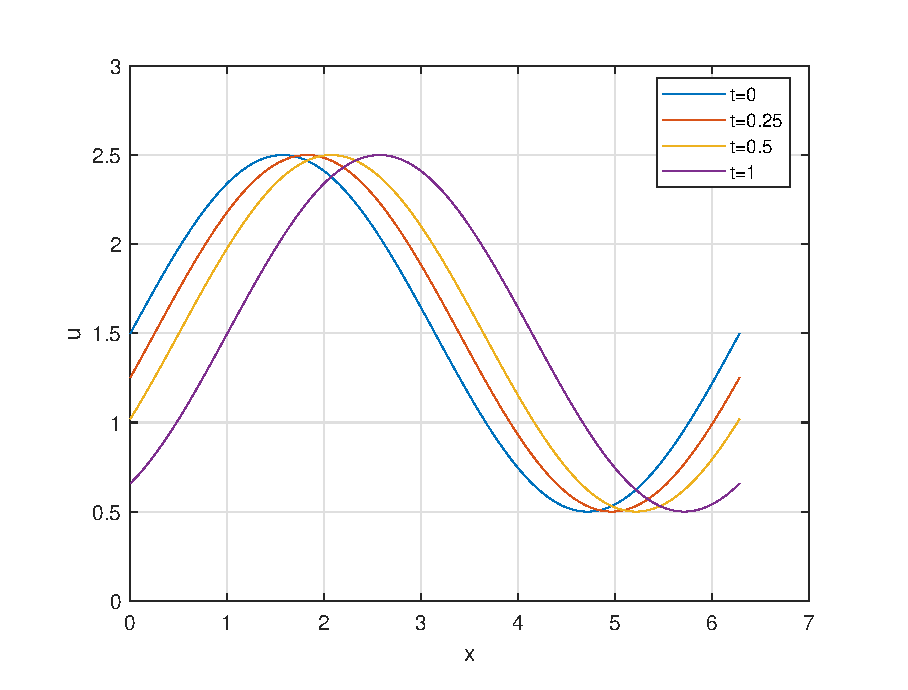
\includegraphics[scale=0.75]{Q1_exactsolution}
\caption{Plot of the analytic solution of the advection equation with the sine-wave initial profile, for the pre-specified times $t=0,0.25,0.5,1$ on the interval $x\in[0,2\pi]$.}
\rule{\linewidth}{.4pt}
\end{figure}
We observe that in plotting the analytic solution of the advection equation with $C=1$, the solution does indeed correspond to a wave travelling to the right as time increases. Now using the discontinuous Galerkin method with linear interpolation, we will check the numerical solution obtained at the specified times $t=0,0.25,0.5,1$. As we are now solving the advection numerically, in order to construct a picture of the function and predict its profile in the future, we are forced to take discrete steps in time and space to approximate the function. In the case of sine-wave initial condition, we are in the continuous setting, therefore we enforce the constraint that the unknown function we are attempting to estimate must take the same value in the neighbouring elements, that is $u^{e-1}_1 = u^{e}_0$. In comparing the numerical solution with the exact solution we can conduct error analysis on the approximation to the exact solution to assess the quality of given numerical solution.\\ 

% how we got to the soln, talk about method ...
% vectors and ode system 
     
  
\begin{figure}[H]
\centering
\rule{\linewidth}{.4pt}
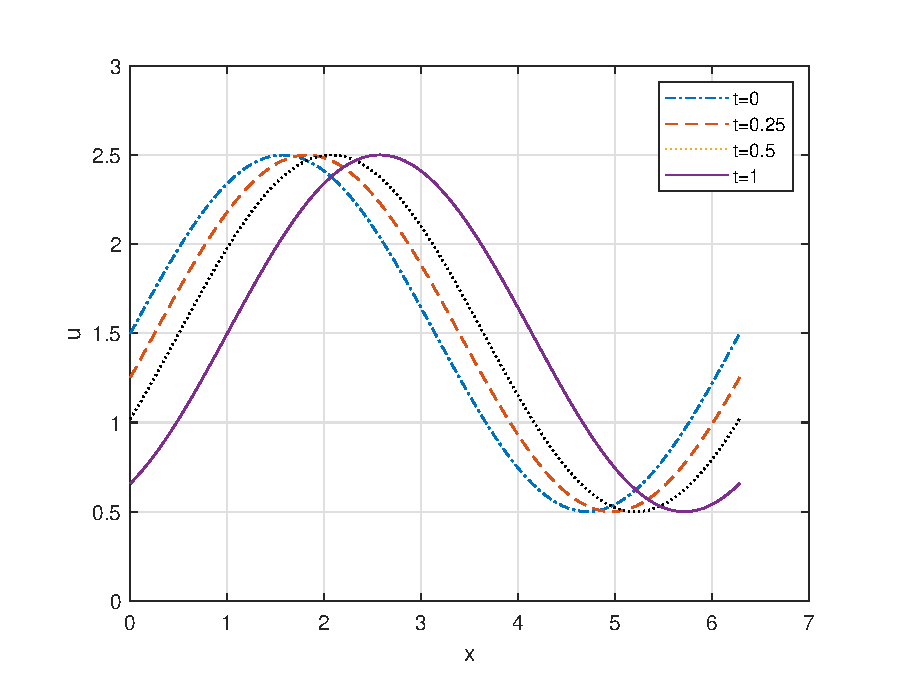
\includegraphics[scale=0.75]{Q1_approximatesolution}
\caption{Numerical solution of the advection equation with sine-wave initial condition for times $t=0,0.25,0.5,1$ on the interval $x\in[0,2\pi]$ with a resolution of timestep $t=0.001$ and $n=100$.}
\rule{\linewidth}{.4pt}  
\end{figure}

We note that in general, the quality of a numerical solution deteriorates as time is increased. Therefore we are required to perform grid and timestep resolution studies to assess the quality of the solution as time is increased. Furthermore as we are comparing the numerical solution with the analytic solution for times up to $t=1$, we need only ensure that the numerical solution is accurate up to $t=1$. In figure 2, the solution obtained using the discontinuous Galerkin method for times $t=0,0.25,0.5,1$ is shown. We observe that with a grid and timestep resolution of $t=0.001$ and $n=100$, the numerical solution appears to be identical. As the quality solution is known to deteriorate as time increases, we can conduct error analysis on the solution at the last timestep $t=1$ to assess the quality of the solution. We find that the maximum deviation of the numerical solution from the exact solution is 0.00082769, hence as the error of the numerical solution at $t=1$ is found to be at most of order $10^{-4}$, we can conclude that this resolution gives a very accurate solution. This is also observed in figure 2 as not only does the shape of the curve appear identical but crucially the curve appears to remain below $u=2.5$ and above $u=0.5$, hence it does not appear to have grown in amplitude as time has increased. This would be a feature of a solution that has decreased in accuracy as time has increased. Below in grid and timestep resolution studies we confirm that this resolution is indeed acceptable. \\   

\begin{figure}[H]
\begin{center}
\rule{\linewidth}{.4pt}
\end{center}
\begin{subfigure}[b]{0.5\textwidth}
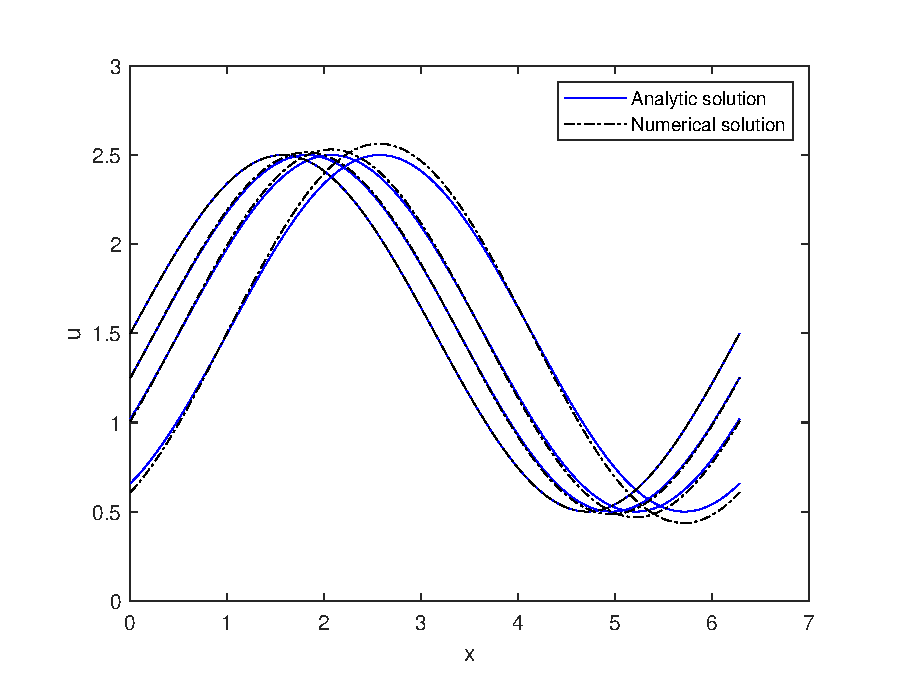
\includegraphics[width=\textwidth]{Q1_t=0.125n=100}\hfill
\caption{Resolution $t=0.125$ and $n=100$.}%Eigenfunction with real and imaginary parts that has corresponding eigenvalue $c_4=0.26402-0.00002i$.}
\end{subfigure}
\begin{subfigure}[b]{0.5\textwidth}
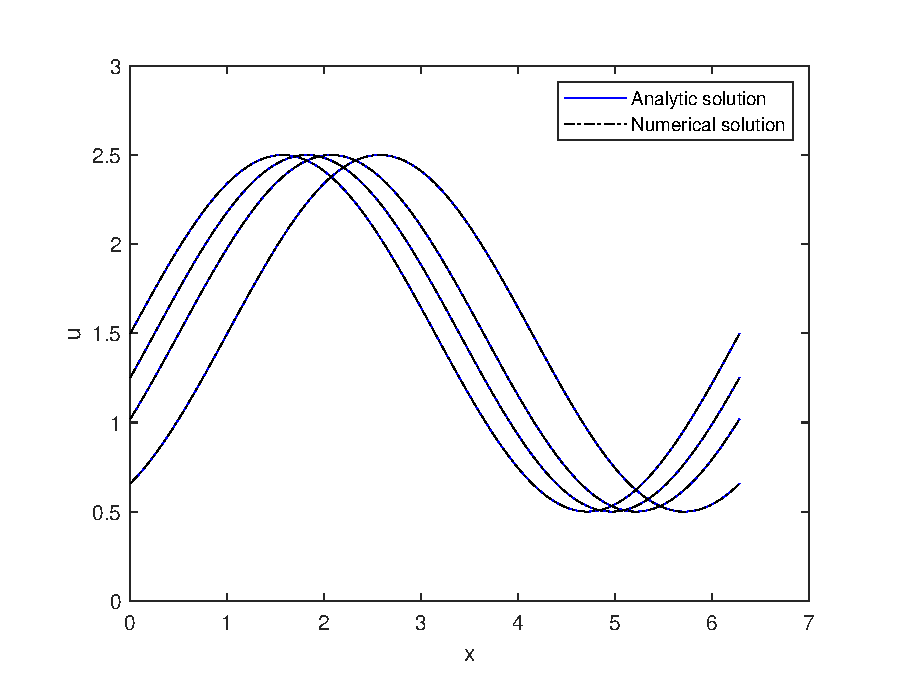
\includegraphics[width=\textwidth]{Q1_t=0.001n=100}\hfill
\caption{Resolution $t=0.001$ and $n=100$.}%Eigenfunction with corresponding eigenvalue $c_{30}=0.70631-0.29852i$.}
\end{subfigure}
\begin{subfigure}[b]{0.5\textwidth}
%\centering
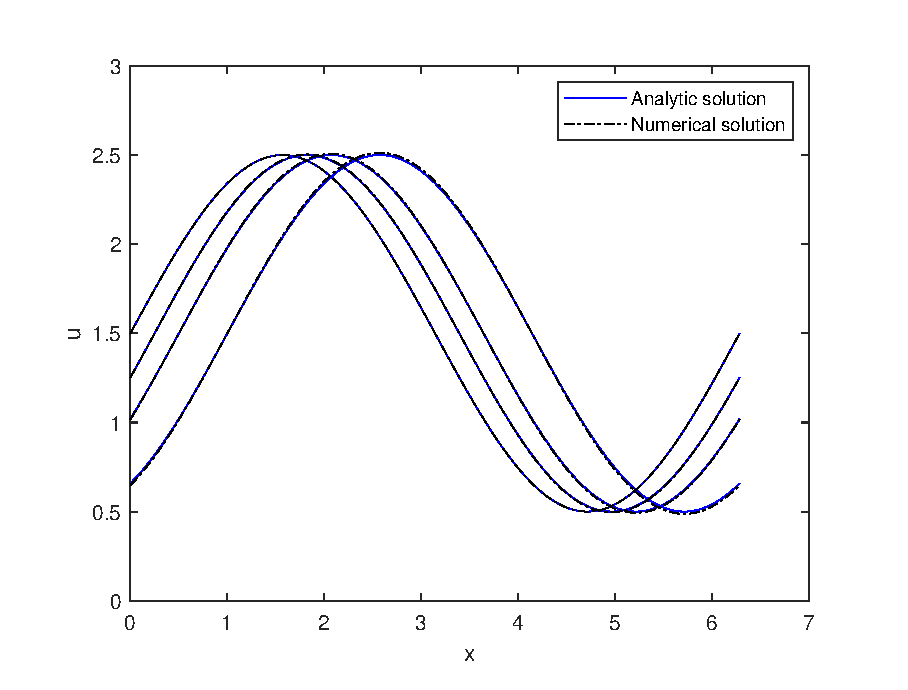
\includegraphics[width=\textwidth]{Q1_t=0.025n=100}\hfill
\caption{Resolution $t=0.025$ and $n=100$.}%Eigenfunction with corresponding eigenvalue $c_{35}=0.67501-0.41198i$.}
\end{subfigure}
\begin{subfigure}[b]{0.5\textwidth}
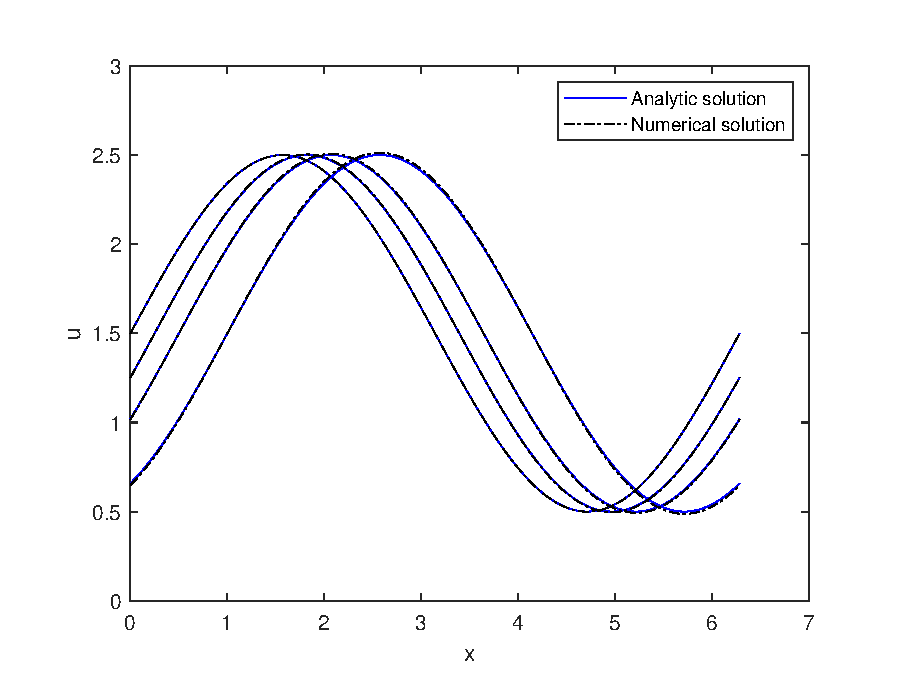
\includegraphics[width=\textwidth]{Q1_t=0.025n=400}\hfill
\caption{Resolution $t=0.025$ and $n=400$.}%Eigenfunction with corresponding eigenvalue $c_{30}=0.70631-0.29852i$.}
\end{subfigure}
\caption{Numerical solution on various resolutions with the analytic solution.}
\rule{\linewidth}{.4pt}
\end{figure}  
In figure 3, we have four plots of the solution to the advection equation obtained using the discontinuous Galerkin method using various resolutions. The four curves in the plots correspond to the times  $t=0,0.25,0.5,1$. Firstly we observe that in figure 3(a), the numerical solution at $t=0.25$ is reasonably accurate as we only see the solution deviate slightly from the exact solution at the peaks and troughs of the curve. However for the subsequent curves corresponding to the times $t=0.5$ and $t=1$ the solution becomes less accurate, deviating more and more from exact solution. At time $t=1$, the maximum error, that is the maximum absolute error of the numerical solution compared with the exact solution, is $0.0642$. In comparison, in figure 3(b), we have a resolution of $t=0.001$ and $n=100$ where we know the maximum absolute error of the numerical solution is $0.00082769$, therefore the error is significantly less with a much smaller timestep. This is also clear when looking at the plot of the numerical solution with the exact solution, the numerical solution is consistently very close to the exact solution and it is very difficult to distinguish between the two solutions up to time $t=1$. \\   
  
We can also consider changing the grid spacing to alter the resolution of our numerical solution. This is shown in figures 3(c) and 3(d). We observe that with a grid and timestep resolution of $t=0.025$ and $n=100$, the numerical solution only noticably deviates from the solution at time $t=0.5$. The plot of numerical solution is also shown again with $t=0.025$ but with $n=400$, thus we have many more elements in our numerical scheme. However increasing the number of grid points does not appear to improve the accuracy of the solution as the maximum absolute error of the numerical solution with these settings is $0.0126$ for both curves. Therefore it would appears that even with four times as many grid points in our numerical scheme, we gain no more accuracy in our solution, and should therefore look to decreasing the timestep in order to obtain a more accurate solution at $t=1$. Clearly however, we do require a sufficient number of grid points, to be able to approximate the solution in the regions of rapid change, for example the peaks and troughs. The resolution settings of $t=0.001$ and $n=100$ do appear to be sufficiently accurate in approximating the exact solution in the region $x\in[0,2\pi]$ for $t=0,0.25,0.5,1$.\\   


% n=100 0.0126
% n= 400   0.0126
  
  
\subsection{Advection equation with square-wave initial condition}

Seondly, we are required to solve the advection equation with a square-wave initial condition given by,
\begin{numcases}{u =}
1 & $0 \leq x \leq 1$ \\
0 & otherwise 
\end{numcases}
Different from the previous initial condition, this condition has a discontinuity at $x=1$, therefore we cannot expect to use the normal function for the flux $f(u)$ to calculate the flux for a given $u$. The initial profile of the square-wave initial condition on our interval $x\in[0,2\pi]$, is given by a horizontal line at $u=1$ from $x=0$ to $x=1$, then $u=0$ for the remainder of the interval. In this case we must make use of the numerical flux, which takes information from adjacent elements. The choice of numerical flux is the local Lax-Friedrichs flux which requires us to calculate the maximum of the derivative over the interval we are calculating the numerical flux. Fortunately, the flux function in this case is $f(u)=u$ with $C=1$, therefore the function is differentiable and the derivative is simply a constant over any interval we wish to calculate the numerical flux. Therefore we can set the maximum of the derivative over the interval to be this constant. \\   
% discontinuity

We can solve the advection equation subject to the initial condition given by the square-wave. This exact solution can then be compared with the numerical solution found by the discontinuous Galerkin method. Firstly we begin by confirming that we do not expect any shocks to appear in the solution to the advection equation. We can check to see if shocks occur by considering a quantity derived from the condition of validity, which states that for a given equation of the form,
\begin{align*}
u_t + c(u)u_x = 0,
\end{align*} 
where in the case of the advection equation the function $c(u)=1$. It it known that the solution takes the form $u=f(\xi)$ on the characteristic curves defined by,
\begin{align*}
x = \xi + tF(\xi),
\end{align*}
where $F(\xi)=c(f(\xi))=1$ in our particular case. Hence the solution takes the form $u=f(\xi)$ on the characteristic curves given by $x = \xi + t$. Now checking for shocks, we consider the quantity $\frac{-1}{F'(\xi)}$ as it is known that if a shock does develop in our solution then it will occur for a given time $t_{crit}$ given by,
\begin{align*}
t_{crit} = \min_{\xi} \left(\frac{-1}{F'(\xi)} \right).
\end{align*}
Hence because $F(\xi)=1$ in our case, the quantity $\frac{-1}{F'(\xi)} = \infty$ always, therefore we do not expect a shock to occur in our solution. Now, in obtaining an analytic solution to the advection equation for the square-wave initial condition, we begin by considering the equation that defines the characteristics $x=\xi +t$, on different regions. Firstly for $\xi \leq 0 \Rightarrow x \leq t$, therefore we expect the solution $u(x,t)=0$ to be valid for $x\leq t$. Secondly, for $0\leq \xi \leq1$ we have $x-t \geq 0$ and $x-t \leq 1$ so we expect the solution $u(x,t)=1$ to be valid on $t\leq x \leq t+1$. Finally for $\xi \geq 1$, we have $x-t \geq 1$ and so $u(x,t)=0$ should be valid on $x\geq 1+t $. The exact solution to the advection equation given the square-wave initial condition is therefore a square-wave which propagates to the right, that has a width of 1 along the $x$-axis. For a given time $t=0.25$ for example, the exact solution takes the form of a square-wave with $u=1$ which begins at $x=0.25$ and ends at $x=1.25$ (and everywhere else zero), hence the amount the wave is shifted by corresponds to the time that has passed. This exact solution can be compared to the numerical solution we shall obtain from the discontinuous Galerkin method. Below plots of the square-wave initial condition are shown as time increases from $t=0$ to $t=1$.\\
 
In figure 4, graphs of the numerical solution to the advection equation using the square-wave initial condition are shown. We observe that the numerical solution does indeed correspond to that of the exact solution calculated above. However there are some artifacts in the neighbourhood of the discontinuities. The graphs of the solution at times $t=0.25,0.5,1$ are still recognisable as a square-wave propagating right along the $x$-axis. For example, at $t=1$ we expect the square-wave to have shifted right by 1 unit in the $x$-direction as the amount the wave is shifted by is equal to the time that has passed, that is $u=1$ on the interval $1\leq x \leq 2$. This is what is observed in figure 3(d), the square-wave does indeed appear to have the profile of $u=1$ on the interval $1\leq x \leq 2$, even if we have the presence of artifacts. Moreover, this is similar to what occurs in figures 3(b) and 3(c), in which the numerical solution using the square-wave initial condition is plotted for times $t=0.25$ and $t=0.5$ respectively.\\ 
 
% intro plot
%plots
\begin{figure}[H]
\begin{center}
\rule{\linewidth}{.4pt}
\end{center}
\begin{subfigure}[b]{0.5\textwidth}
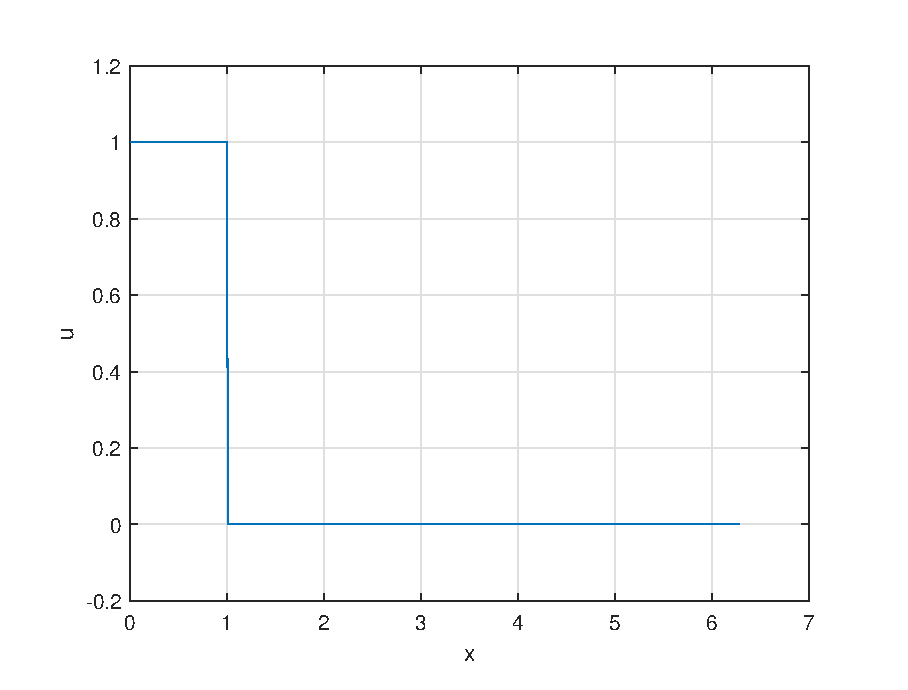
\includegraphics[width=\textwidth]{Q2t=0}\hfill
\caption{Square-wave at time $t=0$.}%Eigenfunction with real and imaginary parts that has corresponding eigenvalue $c_4=0.26402-0.00002i$.}
\end{subfigure}
\begin{subfigure}[b]{0.5\textwidth}
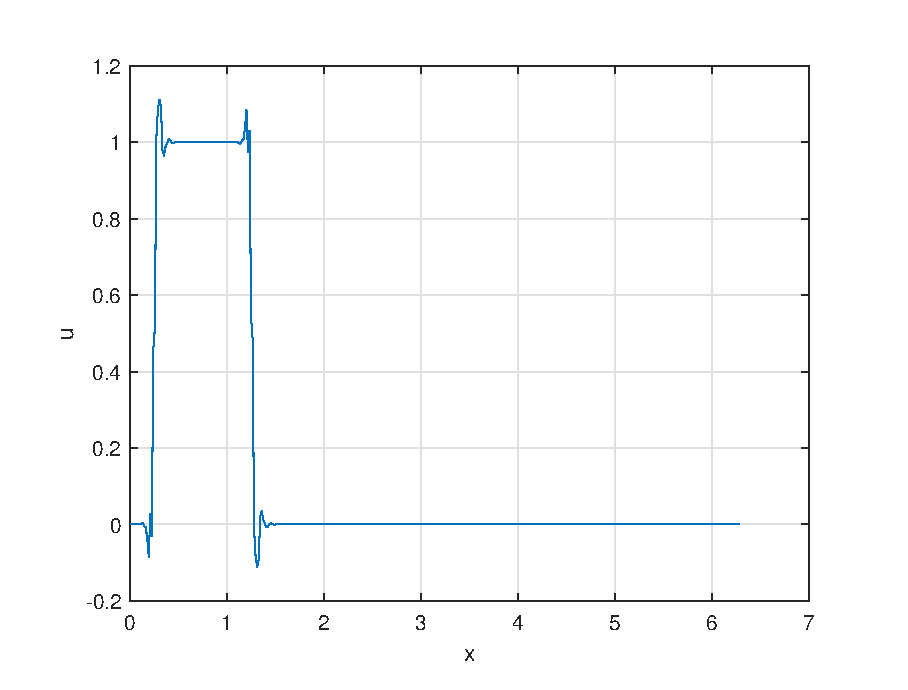
\includegraphics[width=\textwidth]{Q2t=0.25}\hfill
\caption{Square-wave at time $t=0.25$.}%Eigenfunction with corresponding eigenvalue $c_{30}=0.70631-0.29852i$.}
\end{subfigure}
\begin{subfigure}[b]{0.5\textwidth}
%\centering
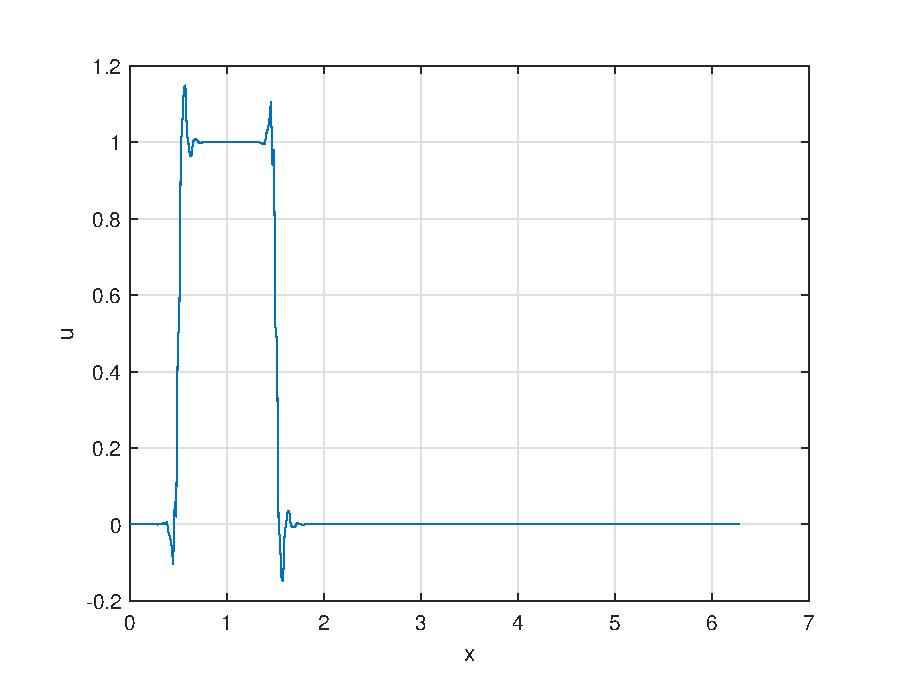
\includegraphics[width=\textwidth]{Q2t=0.5}\hfill
\caption{Square-wave at time $t=0.5$.}%Eigenfunction with corresponding eigenvalue $c_{35}=0.67501-0.41198i$.}
\end{subfigure}
\begin{subfigure}[b]{0.5\textwidth}
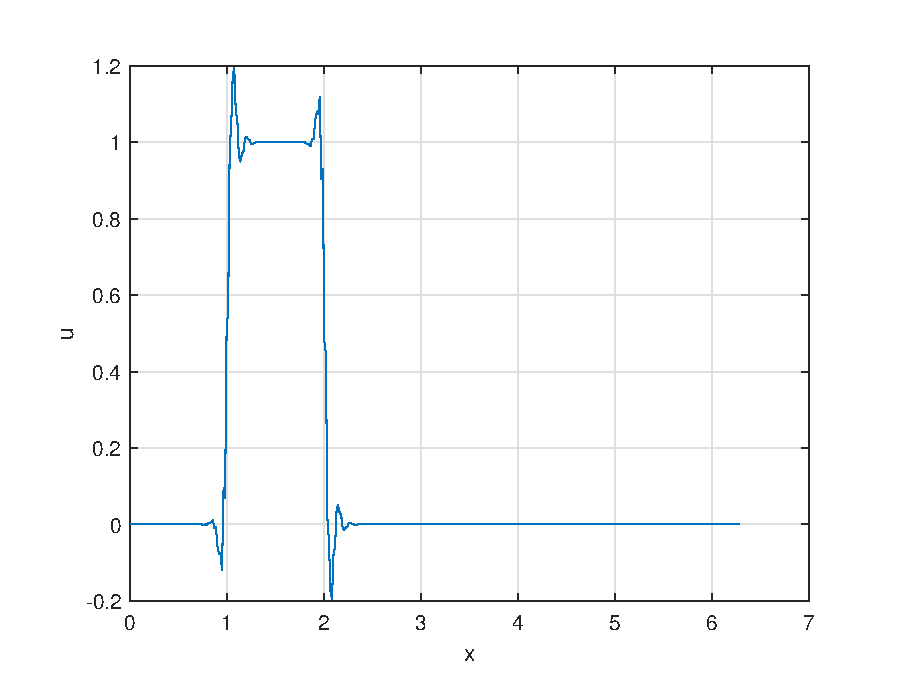
\includegraphics[width=\textwidth]{Q2t=1}\hfill
\caption{Square-wave at time $t=1$.}%Eigenfunction with corresponding eigenvalue $c_{30}=0.70631-0.29852i$.}
\end{subfigure}
\caption{Plots of the square-wave initial condition at the times $t=0,0.25,0.5,1$.}
\rule{\linewidth}{.4pt}
\end{figure}

These graphs of the solution were produced with the resolution of the grid and timestep set to $n=200$ and $t=0.001$. Firstly at $t=0$, we obsere the initial profile of the square-wave. In figure 4(b), we observe that at $t=0.25$ the square-wave appears to have shifted to the right by a small amount and that instead of our solution showing a perfect step function, small artifacts have been introduced at the discontinuities of the square-wave. These artifacts at the discontinuities do not appear to be significant, and they certainly do not appear to dominate the solution but this is clearly no longer a perfect square-wave as seen in the initial profile at $t=0$. In figure 4(c) we observe that at time $t=0.5$, the square-wave has shifted to the right again, and the artifacts do appear to have increased in size by a small amount. If we consider the peak of the artefact at upper left part of the square-wave at time $t=0.25$ (given by $u=1.111$), the small increase in the magnitude between this and the square-wave at $t=0.5$ (given by $u=1.149$) is found to be $0.038$. Hence the artifacts do indeed appear to grow with time. \\     

In figure 4(d), we observe the square-wave has shifted even more to the right and the artifacts in the neighbourhood of the discontinuities have grown again. Although the artifacts have increased in magnitude, we note that at this resolution the artifacts do not appear to dominate and they quickly dissipate. If we were to use a reduced grid and timestep resolution, we could expect the artifacts to dominate as the accuracy of the solution decreases as time increases. Furthermore if we again compare the artefact located at the upper left part of the square-wave, at time $t=1$ this has a value of $u=1.196$, therefore in comparison with the solution at $t=0.5$, the difference in the size of the artifacts is $0.047$. This confirms that at least for $t\in[0,1]$, the artifacts found in the numerical solution to the advection equation obtained by the discontinuous Galerkin method, do not completely dominate the solution. Comparing the increase in the magnitude of the artifacts at $t=0.5$ and $t=0$ (increase=0.149) with that at $t=1$ and $t=0.5$ (increase=0.047), this does not appear to have grown over the interval $t\in[0,1]$. Hence we can conclude that, although the solution has some artifacts around the discontinuities, the structure of the solution does appear to hold for $t\in[0,1]$ as we can still recognise the solution as an imperfect square-wave. \\



% resolution to problem




\subsection{Burgers' equation with sine-wave and square-wave initial condition}

In this section we solve Burgers' equation using the sine-wave initial condition as well as the square-wave initial condition. The difference between Burgers' equation and the advection equation is that $f(u)=\frac{1}{2}u^2$, thus in the implementation of the discontinuous Galerkin method, we use inheritance to create another class named BurgersElement. This class inherits from the AdvectionElement class used previously for solving the advection equation. Therefore we overload the appropriate functions so that BurgersElement applies to Burgers' equation, in order to this the flux and numerical flux are changed as these were the only functions that were defined to be virtual in the AdvectionElement class.    

\subsubsection{Sine-wave initial condition}
Now we will solve Burgers' equation using the sine-wave initial condition used previously to solve the advection equation. Again, we can check to see if we expect a shock to develop in our solution and calculate the time at which we expect this shock to occur. Recall the sine-wave initial condition is given by,
\begin{align*}
u(x,0) = 1.5 + \sin(x).
\end{align*}
In this case the $f(\xi)=1.5+\sin(\xi)$, with c(u)=u and the solution takes the form $u=f(\xi)$ on the characteristic curves given by the equation $x = \xi + tF(\xi)$, where the function $F(\xi) = c(f(\xi))$. If a shock is to occur then it will develop at time $t_{crit}$ given by the following,
\begin{align*}
t_{crit} = \min_{\xi} \left(\frac{-1}{F'(\xi)} \right).
\end{align*} 
In this case we have,
\begin{align*}
t(\xi) &= \frac{-1}{\cos(\xi)},\\ 
\Rightarrow t'(\xi) &= \frac{-\sin(\xi)}{\cos^2(\xi)}.
\end{align*}
We wish to find the minimum of the function $t(\xi)$, hence we set the derivative of the function to zero and we find that derivative is equal to zero for multiplies of $\pi$, that is $t'(\xi)=0$ for $\xi = n\pi, for n\in\mathbb{Z}$. As we require the time to be positive for the time of the shocks to exist, we note that $t(\xi=\pi) = 1$ which minimizes the function. Hence we expect a shock to occur for time given by $t_{crit}=1$. As we have an initial sine-wave profile, we expect the wave to break as the time is increased closer and closer to $t=t_{crit}$. This is because as the wave breaks, $\frac{\partial u}{\partial x}\rightarrow \infty$, thus we expect to observe a discontinuity here. However, because the discontinuous Galerkin method can deal with such shocks, we can expect to see the profile of a different solution for $t>t_{crit}$. Below graphs of the numerical solution to Burgers' equation with the sine-wave initial condition are shown. \\
 
\begin{figure}[H]
\begin{center}
\rule{\linewidth}{.4pt}
\end{center}
\begin{subfigure}[b]{0.5\textwidth}
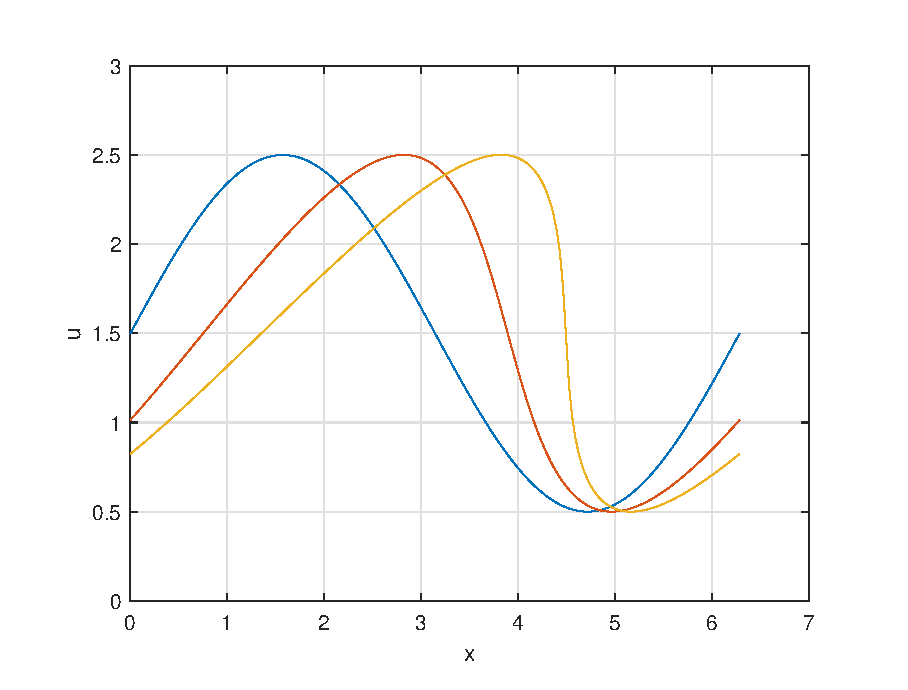
\includegraphics[width=\textwidth]{Q3sine_t=09}\hfill
\caption{Sine-wave at times $t=0,0.5,0.9$.}%Eigenfunction with real and imaginary parts that has corresponding eigenvalue $c_4=0.26402-0.00002i$.}
\end{subfigure}
\begin{subfigure}[b]{0.5\textwidth}
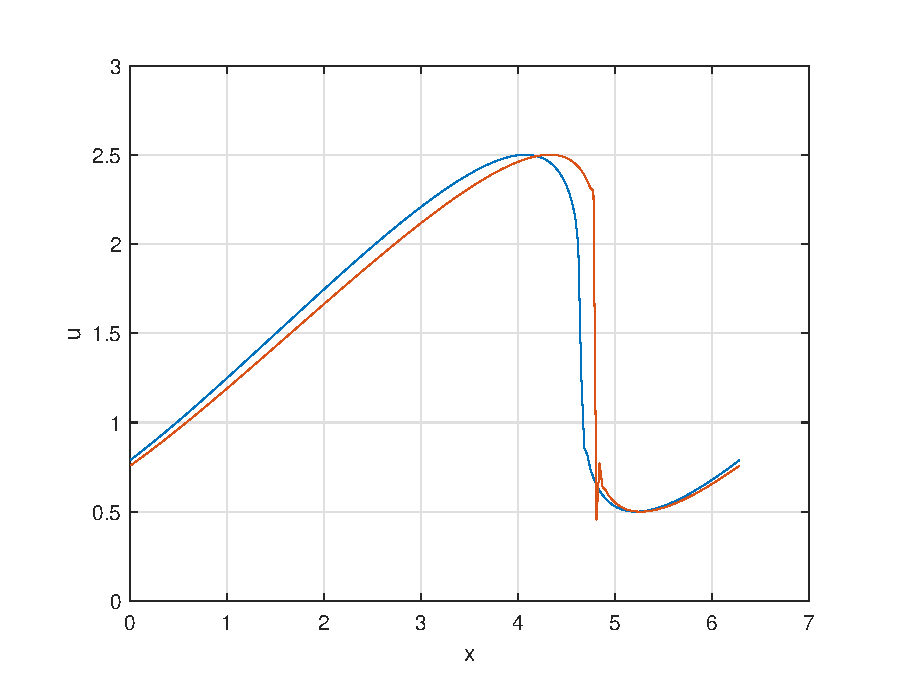
\includegraphics[width=\textwidth]{Q3sine_t=11}\hfill
\caption{Sine-wave at times $t=1,1.1$.}%Eigenfunction with corresponding eigenvalue $c_{30}=0.70631-0.29852i$.}
\end{subfigure}
\begin{subfigure}[b]{0.5\textwidth}
%\centering
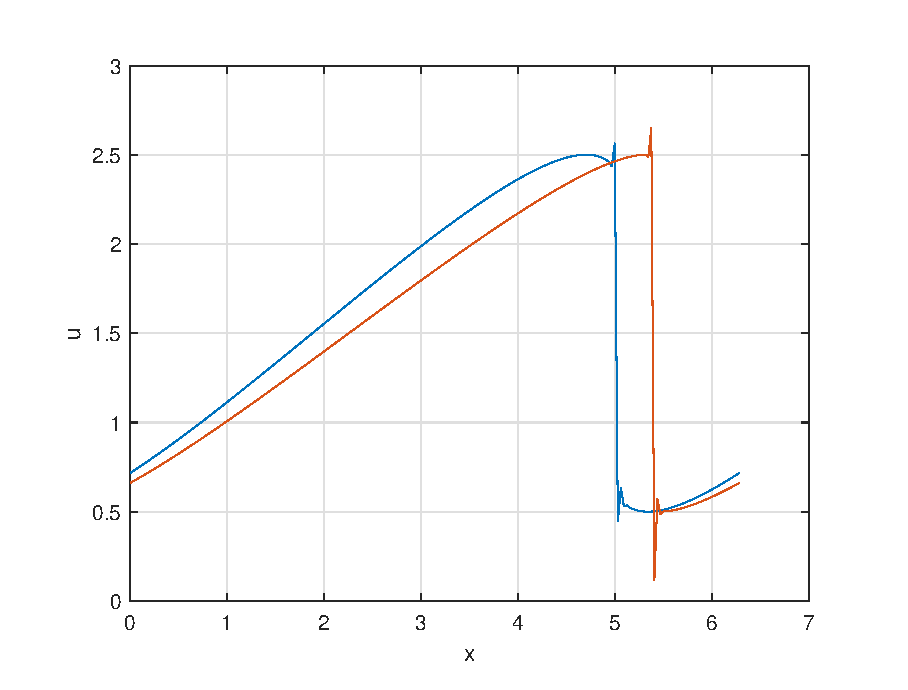
\includegraphics[width=\textwidth]{Q3sine_t=15}\hfill
\caption{Sine-wave at times $t=1.25,1.5$.}%Eigenfunction with corresponding eigenvalue $c_{35}=0.67501-0.41198i$.}
\end{subfigure}
\begin{subfigure}[b]{0.5\textwidth}
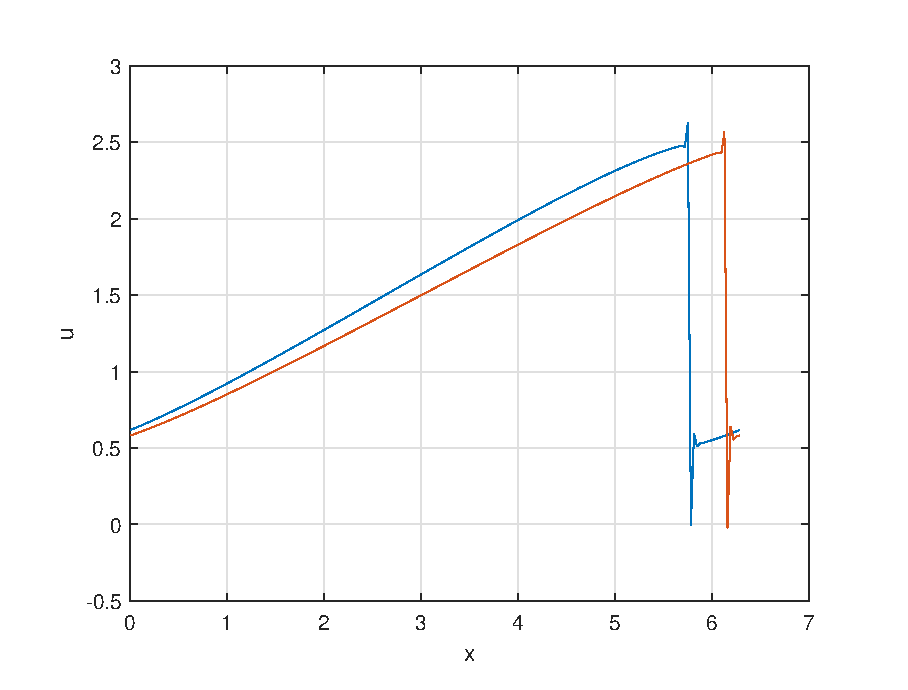
\includegraphics[width=\textwidth]{Q3sine_t=2}\hfill
\caption{Sine-wave at times $t=1.75,2$.}%Eigenfunction with corresponding eigenvalue $c_{30}=0.70631-0.29852i$.}
\end{subfigure}
\caption{Plots of the sine-wave initial condition for various times over the interval $t\in[0,2]$.}
\rule{\linewidth}{.4pt}
\end{figure}

In figure 5, the graphs of numerical solution are shown for $t=0,0.5,0.9,1,1.1,1.25,1.75,2$ allowing us to analyse the behaviour of the initial profile as time increases over the interval $t\in[0,2]$. In figure 5(a), as time increases the initial profile transforms from its initial regular sinusoidal shape to a the shape of a wave breaking, this is demonstrated by the peak of the initial profile shifting to the right and as time increases. It was predicted by the calculations above that a shock would occur for $t=1$. The graphs of the numerical solution confirm this. As time is increased closer to $t=1$, the wave appears to be getting closer to breaking, after this time the function would become triple-valued as the peak of wave overtakes the trough of the curve travelling right. We note that for $t=1$ (the blue curve in figure 3(b)) the curve appears to be smooth with no artifacts in the solution. Whereas for $t=1.1$, there is a small artefact at the lower part of the curve suggesting that the wave has broken as predicted at $t=1$. However because the discontinuous Galerkin method can deal with discontinuities, we observe that for $t>1$ the profile propagates as a discontinuous curve, with the discontinuity travelling right. \\      

The numerical solution illustrated by the graphs in figure 5, corresponds to our analytic predicition that a shock would occur for $t=1$. The discontinuous Galerkin method has therefore successfully allowed us to obtain the solution to Burgers' equation with a sine-wave profile as time increases. An important aspect of a numerical scheme is its stability. We note it was shown that in early numerical models with the discontinuous Galerkin method, making use of an explicit timestepping scheme, were found to be unconditionally unstable unless a very restrictive time step was utilised \cite{LaiKhan2013}. In order to overcome this drawback, other methods were introduced namely the Runge-Kutta Discontinuous method, thus allowing the method to become popularised and used extensively. Hence in this case where the method must deal with the shock which occurs at $t=1$, it is evident that the method remains stable for our choice of timestep.\\    

\subsubsection{Square-wave initial condition}

In this case we are using the square-wave as the initial condition. We can again check to see if we expect there to be any shocks that develop. We begin by recalling the square-wave initial condition,
\begin{numcases}{u =}
1 & $0 \leq x \leq 1$ \\
0 & otherwise 
\end{numcases}
and we wish to solve Burgers' equation subject to this condition on the interval $t\in[0,2]$. We note that $F(\xi) = c(f(\xi)) = f(\xi)$ in this case as $c(u)=u$ in the general form of the following,
\begin{align*}
u_t + c(u)u_x = 0.
\end{align*} 
Again if a shock is to occur then it will develop at time $t_{crit}$ given by the following,
\begin{align*}
t_{crit} = \min_{\xi} \left(\frac{-1}{F'(\xi)} \right).
\end{align*} 
Now, considering the quantity $\frac{-1}{F'(\xi)}$, where $F(\xi)=c'(f(\xi))f'(\xi) = f'(\xi)$. If $\xi<0$ we have that $f(\xi)=f'(\xi)=0$, therefore we have that the quantity is infinite, $\frac{-1}{F'(\xi)}=\infty$. For $\xi$ in the interval $0\leq \xi \leq 1$, we have $f(\xi)=1$ and so $f'(\xi)=0$, resulting again in $\frac{-1}{F'(\xi)}=\infty$. Finally, if $\xi>1$ we have that $f(\xi)=f'(\xi)=0$ just as in the first case. This means that $\frac{-1}{F'(\xi)}=\infty$ in our final region. In summary from these results, we do not expect a shock to form in the interval $t\in[0,2]$. We will assess whether this prediction is true by considering the numerical solution obtained by the discontinuous Galerkin method. Shown below in figure 6 are the plots of the numerical solution at various times in the interval $t\in[0,2]$. 
% graphs
\begin{figure}[H]
\begin{center}
\rule{\linewidth}{.4pt}
\end{center}
\begin{subfigure}[b]{0.5\textwidth}
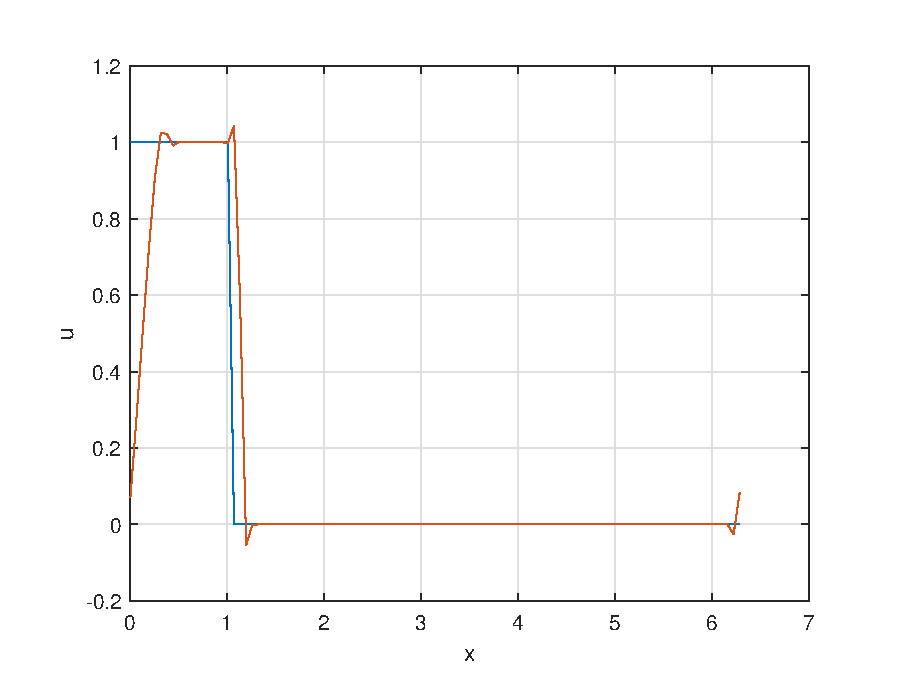
\includegraphics[width=\textwidth]{Q3square_t=025}\hfill
\caption{Square-wave at times $t=0,0.25$.}%Eigenfunction with real and imaginary parts that has corresponding eigenvalue $c_4=0.26402-0.00002i$.}
\end{subfigure}
\begin{subfigure}[b]{0.5\textwidth}
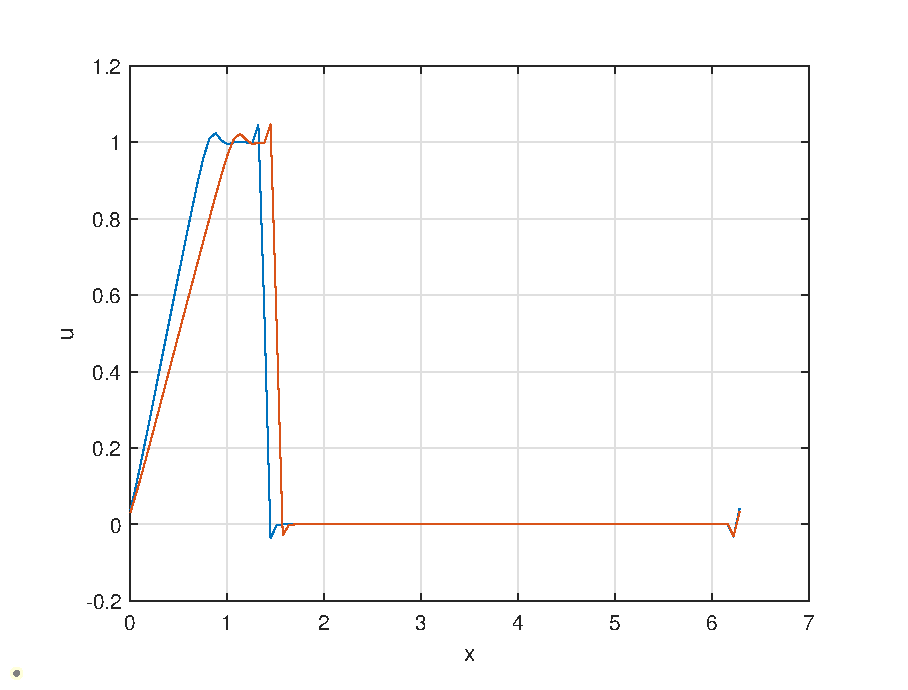
\includegraphics[width=\textwidth]{Q3square_t=1}\hfill
\caption{Square-wave at time $t=0.75,1$.}%Eigenfunction with corresponding eigenvalue $c_{30}=0.70631-0.29852i$.}
\end{subfigure}
\begin{subfigure}[b]{0.5\textwidth}
%\centering
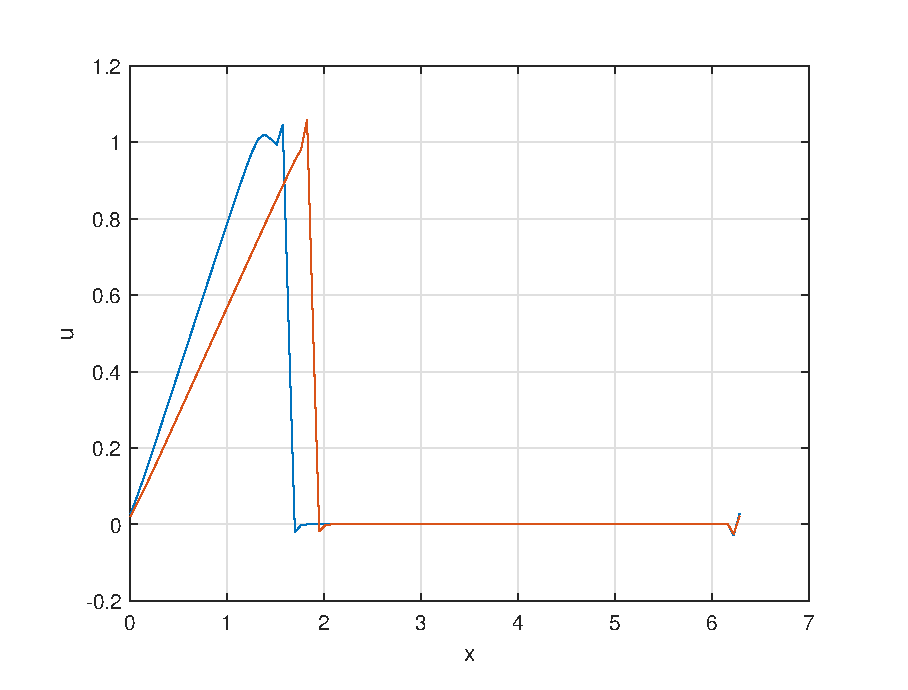
\includegraphics[width=\textwidth]{Q3square_t=175}\hfill
\caption{Square-wave at time $t=1.25,1.75$.}%Eigenfunction with corresponding eigenvalue $c_{35}=0.67501-0.41198i$.}
\end{subfigure}
\begin{subfigure}[b]{0.5\textwidth}
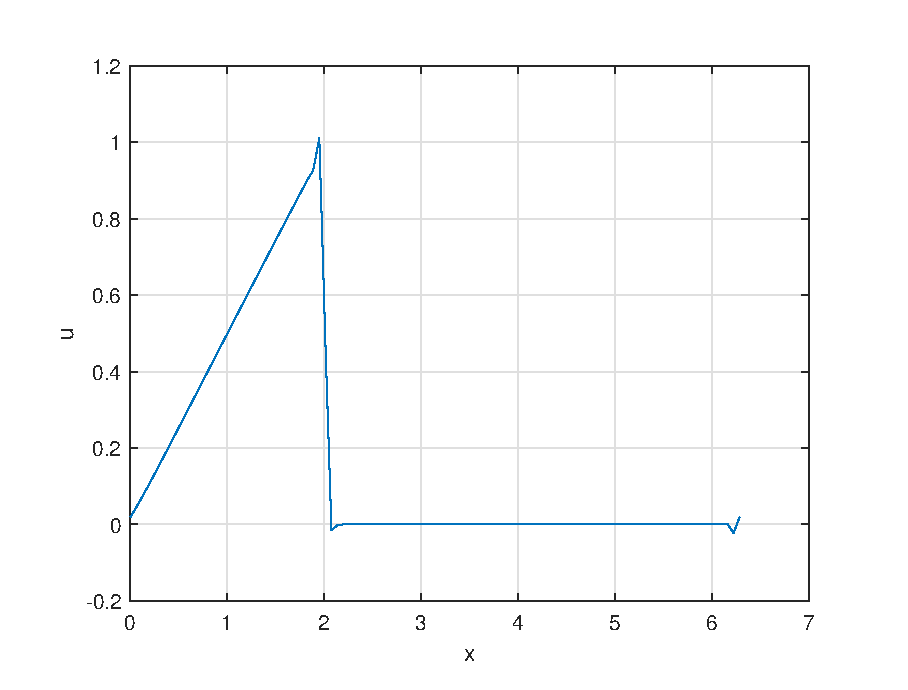
\includegraphics[width=\textwidth]{Q3square_t=2}\hfill
\caption{Square-wave at time $t=2$.}%Eigenfunction with corresponding eigenvalue $c_{30}=0.70631-0.29852i$.}
\end{subfigure}
\caption{Plots of the square-wave initial condition for various times over the interval $t\in[0,2]$.}
\rule{\linewidth}{.4pt}
\end{figure}
% anaylsis on graphs

In figure 6, we have plotted the numerical solution of Burgers' equation subject to the square-wave initial condition. We note that over $t\in[0,2]$ we do not observe a shock forming in the solution, therefore our prediction that a shock would not form is confirmed by this numerical solution. The numerical solution was obtained with a grid and timestep resolution of $t=0.0005$ and $n=200$, which we know should give a sufficiently accurate solution from previous grid and timestep resolution studies. At $t=0$, the solution takes the shape of a square-wave, and we observe that as time increases and the wave propagates to the right, the profile of the wave is no longer square. As we are using the square-wave initial condition, we observe that there are small artifacts again at the discontinuities, however these do not appear to grow with time or dominate the solution. This suggests that the implementation of the discontinuous Galerkin method has been successful in obtaining a numerical solution.\\

  
%
 %
  
  
%=============================================================================================================================
\newpage
\section{Conclusions}
In conclusion the implementation of the discontinuous Galerkin methods has allowed us obtain an accurate numerical solution to the transport equation in the cases of the advection equation and Burgers' equation. It has also been demonstrated that the discontinuous Galerkin method can handle shocks that appear in the solution, this was demonstrated by the sine-wave initial condition for Burgers' equation. The method was also able to confirm predictions made corresponding to the solution and at what time we can expect a shock. It was also found that using the square-wave initial condition, small artifacts are present in the solution in using the discontinuous Galerkin method. These small fluctuations that appear in the solution and can be observed in the graphs of the solution are not naturally present but appear as a result of a diffusion component in the implementation of our method.\\

Furthermore we can conclude that the effect of choosing a grid and timestep resolution that corresponds to an accurate solution is very important for estimating the solution at a given time. Performing grid and timestep resolution studies ensures that we have an accurate solution to the equation. If our resolution resulted in a solution of poor quality, the effects of this are observed most clearly when $t$ is increased. Therefore performing such studies on the resolution are essential in testing the method, to ensure accuracy of the numerical scheme. In this implementation the method was able to cope with the shocks, moreover we were able to verify and validate the analytic solutions and also the predicitions on when the shocks would occur. Hence the discontinuous Galerkin method is a very robust and versatile numerical scheme.\\

\newpage
\begin{thebibliography}{50}
\bibitem[Lai and Khan, 2013]{LaiKhan2013}{\textsc{Lai, W and Khan, A. A} (2013) `Time stepping in discontinuous Galerkin method`, \textit{Journal of Hydrodynamics} \textbf{25}(3), pp321-329.}
\bibitem[Cockburn, \textit{et al.}, 2000]{Cockburn2000}{\textsc{Cockburn, B.\ \textit{et al.}} (2000) `The Development of Discontinuous Galerkin Methods`, \textit{Springer-Verlag}  ,pp3-50.}
\bibitem[Reed and Hill, 1973]{ReedHill1973}{\textsc{Reed, W.\ H. and Hill, T.\ R.}(1973)  `Triangular Mesh Methods for the Neutron Transport Equation`, `Los Alamos`, Scientific Laboratory Report LA-UR-73-479}
\end{thebibliography}




\newpage
\section{Appendix}
AdvectionElement class:
\begin{spverbatim}

class AdvectionElement
{
public:
	// Pointer to the left neighbour
	AdvectionElement* Left_neighbour_pt;
	// Pointer to the right neighbour
	AdvectionElement* Right_neighbour_pt;
	// Storage for the coordinates
	std::vector<double> X;
	// Storage for the unknowns
	std::vector<double> U;
	// Constructor: initialise the vectors to hold two entries.
	AdvectionElement()
	{
		// Resize the vectors to hold two entries each
		X.resize(2);
		U.resize(2);
	}
	// Return the value of the coordinate at local coordinate s using
	// equation (1.2)
	double interpolated_x(double s)
	{
		double psi_0 = 0.5 * (1 - s);
		double psi_1 = 0.5 * (1 + s);
		return X[0] * psi_0 + X[1] * psi_1;
	}
	// Return the value of the unknown at local coordinate s using
	// equation (1.4)
	double interpolated_u(double s)
	{
		return U[0] * 0.5 * (1 - s) + U[1] * 0.5 * (1 + s);
	}
	// ================  Timestepping loop   ===================
	virtual double flux(double u)  // This is a virtual fn so it can be overloaded later
	{
		if (u == interpolated_u(-1.0)) { u = -1.0; }
		else if (u == interpolated_u(1.0)) { u = 1.0; }
		else {
			if (u>U[0] && u<U[1])
			{
				double s = (2 * u - (U[0] + U[1])) / (U[1] - U[0]); // This doesn't work if using a discontinuous IC
				//std::cout << "s= " << s << std::endl;
				u=s;
			}
			else {
				return u; // "inbetween elements"
			}
		}
		double returnVal = interpolated_u(u); // f(u)=u
		return returnVal;
	}
	// A function that returns the integral of the flux function over the element using two-point Gauss rule
	double integrate_flux()
	{
		// Using two-point Gauss rule
		return flux(interpolated_u(-1.0 / sqrt(3))) + flux(interpolated_u(1.0 / sqrt(3)));
	}
	// A function h(a,b) that returns the numerical flux. Local Lax-Friedrichs flux
	virtual double h(double a, double b)
	{
		// Lax-Friedrichs flux
		double max = 1.0;
		// Return the quantity 
		return 0.5 * (flux(a) + flux(b)) - 0.5 * max * (b - a);
	}
	MVector U_updated;
	// A function that calculates the updated values of the unknowns U using first-order scheme
	void timestep(double dt)
	{
		MVector U_timestep(2),Flux(2),F_e(2),U_;
		MMatrix M_e(2,2,0.0);
		double coef = (X[1] - X[0]) / 6;
		M_e(0, 0) = coef * 2.0;
		M_e(0, 1) = M_e(1, 0) = coef * 1.0;
		M_e(1, 1) = coef * 2.0;
		F_e[0] = -0.5 * integrate_flux();
		F_e[1] = 0.5 * integrate_flux();
		U_ = { U[0],U[1] };
		if ((*Left_neighbour_pt).U[1] == U[0])
		{
			// Continuous
			Flux[0] = flux(U_[0]);
		}
		else
		{
			// Discontinuous
			Flux[0] = h((*Left_neighbour_pt).U[1], U[0]);
		}
		if ((*Right_neighbour_pt).U[0] == U[1])
		{
			// Continuous
			Flux[1] = -flux(U[1]);
		}
		else
		{
			// Discontinuous
			Flux[1] = -h(U[1],(*Right_neighbour_pt).U[0]);
		}
		// Vector equation which calculates updates
		U_timestep = U_ + dt *( M_e.invert(M_e) * (F_e+Flux));
		U_updated=U_timestep;
	}
	
}; //End of the class definition
\end{spverbatim}

BurgersElements class:
\begin{spverbatim}
// ===   Derived class   ===
// Creating a new class called BurgersElement, which is required to solve Burger's equation using discontinuous Galerkin
// methods. The approriate flux and numerical flux function need to be overloaded for this to work!
class BurgersElement : public AdvectionElement
{
	// This BurgersElement inherits from the AdvectionElements class
public:
	// Add existing members function from base class
		// Pointer to the left neighbour
	BurgersElement* Left_neighbour_pt;
	// Pointer to the right neighbour
	BurgersElement* Right_neighbour_pt;
	// Storage for the coordinates
	std::vector<double> X;
	// Storage for the unknowns
	std::vector<double> U;
	// Constructor: initialise the vectors to hold two entries.
	BurgersElement()
	{
		// Resize the vectors to hold two entries each
		X.resize(2);
		U.resize(2);
	}
	// Return the value of the coordinate at local coordinate s using
	// equation (1.2)
	double interpolated_x(double s)
	{
		double psi_0 = 0.5 * (1 - s);
		double psi_1 = 0.5 * (1 + s);
		return X[0] * psi_0 + X[1] * psi_1;
	}
	// Return the value of the unknown at local coordinate s using
	// equation (1.4)
	double interpolated_u(double s)
	{
		return U[0] * 0.5 * (1 - s) + U[1] * 0.5 * (1 + s);
	}
	// ================  Timestepping loop   ===================
	virtual double flux(double u) 
	{
		if (u == interpolated_u(-1.0)) { u = -1.0; }
		else if (u == interpolated_u(1.0)) { u=1.0; }
		else { return 0.5 * pow(u, 2); 

		}
		double returnVal = 0.5*pow(interpolated_u(u), 2);
		return returnVal;
	}
	// A function that returns the integral of the fluz function over the element using two-point Gauss rule
	double integrate_flux()
	{
		// Using two-point Gauss rule
		return flux(interpolated_u(-1.0 / sqrt(3.0))) + flux(interpolated_u(1.0 / sqrt(3.0)));
	}
	// A function h(a,b) that returns the numerical flux. Local Lax-Friedrichs flux 
	virtual double h(double a, double b)
	{
		std::vector<double> v = { std::abs(a), std::abs(b) };
		double max = 0.0;
		for (int i = 0; i < v.size(); i++)
		{
			if (v[i] > max)
			{
				max = v[i];
			}
		}
		// Return the quantity std::cout << 0.5 * (flux(a) + flux(b)) - 0.5 * max * (b - a) << std::endl;
		return 0.5 * (flux(a) + flux(b)) - 0.5 * max * (b - a);
	}
	MVector U_updated;
	// A function that calculates the updated values of the unknowns U using first-order scheme
	void timestep(double dt)
	{
		MVector U_timestep(2), Flux(2), F_e(2), U_;
		MMatrix M_e(2, 2, 0.0);
		double coef = (X[1] - X[0]) / 6;
		M_e(0, 0) = coef * 2.0;
		M_e(0, 1) = M_e(1, 0) = coef * 1.0;
		M_e(1, 1) = coef * 2.0;
		F_e[0] = -0.5 * integrate_flux();
		F_e[1] = 0.5 * integrate_flux();
		U_ = { U[0], U[1] };
		if ((*Left_neighbour_pt).U[1] == U[0])
		{
			// Continuous
			Flux[0] = flux(U_[0]);
		}
		else
		{
			// Discontinuous
			Flux[0] = h((*Left_neighbour_pt).U[1], U[0]);
		}
		if ((*Right_neighbour_pt).U[0] == U[1])
		{
			// Continuous
			Flux[1] = -flux(U_[1]);
		}
		else
		{
			// Discontinuous
			Flux[1] = -h(U[1],(*Right_neighbour_pt).U[0]);
		}
		// Vector equation which calculates updates
		U_timestep = U_ + dt * (M_e.invert(M_e) * (F_e + Flux));
		//display_MVector(dt * (M_e.invert(M_e) * (F_e + Flux)));
		U_updated = U_timestep;
	}
}; // End of class defninition

\end{spverbatim}

Example of implementation of method; Obtaining the numerical solution of Burgers' equation using the square-wave initial condition.

\begin{spverbatim}
	// =======================================       Question 3  -  Discontinuous profile       =============================================
	// Discontinuous initial profile
	int N = 100;
	double x_start = 0.0, x_end = 2 * std::acos(-1.0);
	std::vector<BurgersElement> elements(N);
	for (int j = 0; j < N; j++)
	{
		// Loop over vector to fill out member data X, U
		// Initialise X values
		elements[j].X[0] = x_start + j * (x_end - x_start) / N;
		elements[j].X[1] = x_start + (j + 1) * (x_end - x_start) / N;
		// Using square-wave profile
		if (elements[j].X[0] >= 0.0 && elements[j].X[0] <= 1.0)
		{
			elements[j].U[0] = 1.0;
			elements[j].U[1] = 1.0;
		}
		else
		{
			//std::cout << "Discontinuity occurs at " << j << std::endl;
			elements[j].U[0] = 0.0;
			elements[j].U[1] = 0.0;
		}

	}
	//elements[N - 1].U[1] = elements[0].U[0];  // Connecting the first and last elements U^0_0 = U^{N-1}_1
	for (int i = 0; i < N; i++)
	{
		// Setting neighbour pointers for each element
		if (i == 0)
		{
			// set neighbour pointer connecting first and last element
			elements[i].Left_neighbour_pt = &elements[N - 1];
			elements[i].Right_neighbour_pt = &elements[i + 1];
		}
		else if (i == N - 1)
		{
			// set neighbour pointer connecting first and last element
			elements[i].Right_neighbour_pt = &elements[0];
			elements[i].Left_neighbour_pt = &elements[i - 1];
		}
		else
		{
			elements[i].Left_neighbour_pt = &elements[i - 1];// Left pointer
			elements[i].Right_neighbour_pt = &elements[i + 1];// Right pointer
		}
	}


	//std::cout << elements[15].U[1] << std::endl; // =1
	//std::cout << elements[16].U[0] << std::endl; // =0

	//std::cout << elements[16].Left_neighbour_pt->U[1] << std::endl;
	//std::cout << elements[16].U[0] << std::endl;
	//std::cout << elements[0].flux((elements[16].U[0] + elements[15].Left_neighbour_pt->U[1])/2) << std::endl;
	//std::cout << elements[0].h(elements[15].Left_neighbour_pt->U[1], elements[16].U[0]) << std::endl;
	//elements[16].timestep(0.001);
	//std::cout << elements[16].U_updated[0] << std::endl;


	double dt = 0.0005, total_time=0.0;
	for (int k = 0; k < 4000; k++)
	{
		if (k == 0) //t=0
		{
			std::cout << "=========   " << total_time << "   ============" << std::endl;
			std::ofstream Q3square0;
			Q3square0.open("Q3square0.txt");
			if (!Q3square0)
			{
				std::cout << "Couldn't open file!!" << std::endl;
				return 1;
			}
			Q3square0 << elements[0].U[0] << std::endl;
			for (int i = 0; i < N; i++)// Write to file
			{
				//Q3square0 << elements[i].U[0] << std::endl;
				Q3square0 << elements[i].U[1] << std::endl;
			}
			Q3square0.close();
		}
		for (int i = 0; i < N; i++)
		{
			elements[i].timestep(dt);
		}
		for (int j = 0; j < N; j++)
		{
			elements[j].U[0] = elements[j].U_updated[0];
			elements[j].U[1] = elements[j].U_updated[1];
		}
		total_time = total_time + dt;

		/*
		double u_int = 0.0;
		for (int l = 0; l < N - 1; l++)
		{
			u_int = 0.5 * (elements[l].U[1] + elements[l + 1].U[0]);
			elements[l].U[1] = u_int;
			elements[l + 1].U[0] = u_int;
		}*/
		if (k == 499) //t=0.25
		{
			std::cout << "=========   " << total_time << "   ============" << std::endl;
			std::ofstream Q3square025;
			Q3square025.open("Q3square025.txt");
			if (!Q3square025)
			{
				std::cout << "Couldn't open file!!" << std::endl;
				return 1;
			}
			Q3square025 << elements[0].U[0] << std::endl;
			for (int i = 0; i < N; i++)// Write to file
			{
				//Q3square025 << elements[i].U[0] << std::endl;
				Q3square025 << elements[i].U[1] << std::endl;
			}
			Q3square025.close();
		}
		if (k == 1499) //t=0.75
		{
			std::cout << "=========   " << total_time << "   ============" << std::endl;
			std::ofstream Q3square075;
			Q3square075.open("Q3square075.txt");
			if (!Q3square075)
			{
				std::cout << "Couldn't open file!!" << std::endl;
				return 1;
			}
			Q3square075 << elements[0].U[0] << std::endl;
			for (int i = 0; i < N; i++)// Write to file
			{
				//Q3square075 << elements[i].U[0] << std::endl;
				Q3square075 << elements[i].U[1] << std::endl;
			}
			Q3square075.close();
		}
		if (k == 1999) //t=1
		{
			std::cout << "=========   " << total_time << "   ============" << std::endl;
			std::ofstream Q3square1;
			Q3square1.open("Q3square1.txt");
			if (!Q3square1)
			{
				std::cout << "Couldn't open file!!" << std::endl;
				return 1;
			}
			Q3square1 << elements[0].U[0] << std::endl;
			for (int i = 0; i < N; i++)// Write to file
			{
				//Q3square1 << elements[i].U[0] << std::endl;
				Q3square1 << elements[i].U[1] << std::endl;
			}
			Q3square1.close();
		}

		if (k == 2499) //t=1.25
		{
			std::cout << "=========   " << total_time << "   ============" << std::endl;
			std::ofstream Q3square125;
			Q3square125.open("Q3square125.txt");
			if (!Q3square125)
			{
				std::cout << "Couldn't open file!!" << std::endl;
				return 1;
			}
			Q3square125 << elements[0].U[0] << std::endl;
			for (int i = 0; i < N; i++)// Write to file
			{
				//Q3square125 << elements[i].U[0] << std::endl;
				Q3square125 << elements[i].U[1] << std::endl;
			}
			Q3square125.close();
		}

		if (k == 3499) //t=1.75
		{
			std::cout << "=========   " << total_time << "   ============" << std::endl;
			std::ofstream Q3square175;
			Q3square175.open("Q3square175.txt");
			if (!Q3square175)
			{
				std::cout << "Couldn't open file!!" << std::endl;
				return 1;
			}
			Q3square175 << elements[0].U[0] << std::endl;
			for (int i = 0; i < N; i++)// Write to file
			{
				//Q3square1 << elements[i].U[0] << std::endl;
				Q3square175 << elements[i].U[1] << std::endl;
			}
			Q3square175.close();
		}

		if (k == 3999) //t=2
		{
			std::cout << "=========   " << total_time << "   ============" << std::endl;
			std::ofstream Q3square2;
			Q3square2.open("Q3square2.txt");
			if (!Q3square2)
			{
				std::cout << "Couldn't open file!!" << std::endl;
				return 1;
			}
			Q3square2 << elements[0].U[0] << std::endl;
			for (int i = 0; i < N; i++)// Write to file
			{
				//Q3square2 << elements[i].U[0] << std::endl;
				Q3square2 << elements[i].U[1] << std::endl;
			}
			Q3square2.close();
		}

	}
\end{spverbatim}















































\end{document} %==================================================================================================================



